Сессии

HTTP является протоколом без состояния. И хотя некоторые рассматривают это как недостаток, сторонники RESTful веб-разработки восхваляют это как плюс. Ведь когда состояние удалено из общей картины, тогда легче масштабировать приложения, кэширование может происходить автоматически, и доступны многие другие приятные побочные эффекты. Вы можете провести много параллелей с неизменяемой природой Haskell в целом.

Насколько это возможно, RESTful приложениям следует избегать сохранять состояние с информацией о взаимодействии с клиентом. Тем не менее, иногда это неизбежно. Такая функциональность как корзина покупок является классическим примером, но другие более обычные взаимодействия, наподобие должной обработки входа в систему, могут быть значительно улучшены путем правильного использования сессий.

В этой главе описывается, как Yesod сохраняет данные сессии, как вы можете получить доступ к этим данным, а также некоторые специальные функции, которые помогут вам использовать сессии наилучшим образом.

Clientsession

Одним из первых пакетов которые отделились от Yesod был clientsession. Этот пакет использует шифрование и подписи для хранения данных в куки-файлах на стороне клиента. Шифрование препятствует пользователю изучать данные, а подпись гарантирует, что сессия не была ни захвачена, ни изменена.

Возможно, с точки зрения эффективности, хранение данных в куки звучит как плохая идея: ведь, это означает, что данные должны быть отправлены на каждый запрос. Однако на практике, clientsession может значительно улучшить производительность.

* Для обслуживания запроса не требуется обращаться к базе данных на стороне сервера.
* Легко масштабировать по горизонтали: каждый запрос содержит всю информацию, необходимую для ответа.
* Для того чтобы уменьщить нагрузку на канал, сайты могут предоставлять статический контент с отдельного доменного имени, чтобы избежать накладных расходов на передачу куки для каждого запроса.

Сохранение мегабайт информации в сессии будет плохой идеей. И поэтому большинство рекомендаций по реализаций сессий не рекомендуют такую практику. Если вам действительно нужно сберегать много данных для пользователя, то лучше хранить ключ поиска в сессии, а фактические данные в базе данных.

Все взаимодействия с clientsession обрабатывается внутри Yesod, но есть несколько мест, где вы можете немного настроить его поведение.

Управление сессиями

В классе типов Yesod существуют три функции, которые управляют работой сессий. Функция encryptKey возвращает текущий ключ шифрования. По умолчанию, она берёт его из локального файла, что бы сессии могли сохраняться между перезагрузками базы данных. Если этот файл не существует, то он будет автоматически создан и заполнен случайными данными. А если переопределить эту функцию, так чтобы она возвращала Nothing, то сессии будут отключены.

Зачем отключать сессии? Они вносят накладные расходы на производительность. При нормальных обстоятельствах, эти расходы минимальны, особенно по сравнению с доступом к базе данных. Однако, когда имеешь дело с очень простыми задачами, эти накладные расходы могут стать заметными. Но будьте осторожны с отключением сессий: ведь это также отключит такую функциональность, как защиту от подделки межсайтовых запросов (Cross-Site Request Forgery, сокращённо CSRF).

Следующая функция clientSessionDuration. Эта функция возвращает количество минут, в течении которых сессия должна быть активной. Значение по умолчанию составляет 120 (2 часа).

Это значение в конечном итоге влияет на куки сессии двумя способами: во-первых, оно определяет срок действия самого куки. Однако, что более важно, время окончания сессии закодирована внутри подписи сессии. Когда Yesod расшифровывает подпись, он проверяет в прошлом ли дата, и если да, то значения сессии игнорируються.

Каждый раз, когда Yesod посылает ответ клиенту, он отправляет обновленное куки с новым сроком годности. Таким образом, даже если вы не изменяете сами значения сессии, срок сессии не истечёт, если пользователь просто продолжает просматривать ваш сайт.

И это подводит к последней функции: sessionIpAddress. По умолчанию, чтобы предотвратить перехват сессии, Yesod также кодирует в куки IP-адрес клиента. В общем, это хорошая вещь. Тем не менее, некоторые провайдеры держат своих пользователей за прокси серверами, которые переписывают их IP-адреса, иногда меняя исходный адресс в середине сессии. Если это произойдет, и sessionIpAddress включен, то сессия пользователя будет сброшена. Установка же этого параметра в False позволит сессии продолжать в таких условиях, ценой подвержения пользователя возможному захвату сессии.

Действия с сессией

Как и большинство фреймворков, сессии в Yesod представляет собой хранилище пар ключ-значение. API базовой сессии сводится к четырем функциям: lookupSession получает значение для ключа (если имеется), getSession возвращает все пары ключ/значение, setSession задаёт значение для ключа, а deleteSession очищает значение для ключа.

\begin{lstlisting}
{-# LANGUAGE TypeFamilies, QuasiQuotes, TemplateHaskell, MultiParamTypeClasses, OverloadedStrings #-}
import Yesod
import Control.Applicative ((<$>), (<*>))
import qualified Web.ClientSession as CS

data SessionExample = SessionExample

mkYesod "SessionExample" [parseRoutes|
/ Root GET POST
|]

getRoot :: Handler RepHtml
getRoot = do
    sess <- getSession
    hamletToRepHtml [hamlet|
<form method=post>
    <input type=text name=key>
    <input type=text name=val>
    <input type=submit>
<h1>#{show sess}
|]

postRoot :: Handler ()
postRoot = do
    (key, mval) <- runInputPost $ (,) <$> ireq textField "key" <*> iopt textField "val"
    case mval of
        Nothing -> deleteSession key
        Just val -> setSession key val
    liftIO $ print (key, mval)
    redirect Root

instance Yesod SessionExample where
    -- Устанавливаем тайм-аут сессии в 1 минуту, что бы облегчить тестирование
    makeSessionBackend _ = do
        key <- CS.getKey CS.defaultKeyFile
        return $ Just $ clientSessionBackend key 1

instance RenderMessage SessionExample FormMessage where
    renderMessage _ _ = defaultFormMessage

main :: IO ()
main = warpDebug 3000 SessionExample
\end{lstlisting}

Сообщения

Одно из использований упомянутых ранее сессий это сообщения. Они используются, чтобы решить одну из обычеых проблем в веб-разработке: пользователь выполняет POST запрос, веб-приложение делает изменения, а затем веб-приложение хочет одновременно перенаправить пользователя на новую страницу и отправить пользователю сообщение об успехе. (Это известно как Post/Redirect/Get).

Yesod предоставляет пару функций, чтобы сделать это очень просто: setMessage сохраняет значение в сессии, и getMessage которая одновременно считывает последнее значение в сессии, и очищает старое значение, так что оно не будет случайно отображаться два раза. 

Рекомендуется вызовать getMessage в defaultLayout, так любое доступное сообщение покажеться пользователю немедленно, без необходимости помнить о добавлениии вызова getMessage в каждый обработчик. 

\begin{lstlisting}
{-# LANGUAGE OverloadedStrings, TypeFamilies, TemplateHaskell,
             QuasiQuotes, MultiParamTypeClasses #-}

import Yesod

data Messages = Messages

mkYesod "Messages" [parseRoutes|
/ RootR GET
/set-message SetMessageR POST
|]

instance Yesod Messages where
    defaultLayout widget = do
        pc <- widgetToPageContent widget
        mmsg <- getMessage
        hamletToRepHtml [hamlet|
$doctype 5
<html>
    <head>
        <title>#{pageTitle pc}
        ^{pageHead pc}
    <body>
        $maybe msg <- mmsg
            <p>Your message was: #{msg}
        ^{pageBody pc}
|]

instance RenderMessage Messages FormMessage where
    renderMessage _ _ = defaultFormMessage

getRootR :: Handler RepHtml
getRootR = defaultLayout [whamlet|
<form method=post action=@{SetMessageR}>
    My message is: #
    <input type=text name=message>
    <input type=submit>
|]

postSetMessageR :: Handler ()
postSetMessageR = do
    msg <- runInputPost $ ireq textField "message"
    setMessage $ toHtml msg
    redirect RootR

main :: IO ()
main = warpDebug 3000 Messages
\end{lstlisting}

\begin{figure}[tbh]
  \centering
  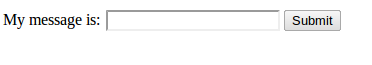
\includegraphics{09-sessions-image-01.png}
  \caption{Первая загрузка страницы, нет сообщения}
\end{figure}

\begin{figure}[tbh]
  \centering
  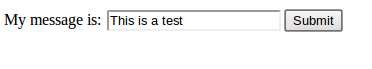
\includegraphics{09-sessions-image-02.png}
  \caption{Новое сообщение введено в текстовое поле}
\end{figure}

\begin{figure}[tbh]
  \centering
  \caption{После отправки формы, сообщение появляется в верхней части страницы}
  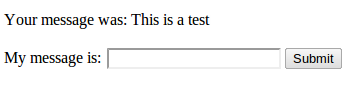
\includegraphics{09-sessions-image-03.png}
\end{figure}

\begin{figure}[tbh]
  \centering
  \caption{После обновления, сообщение очищено}
  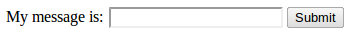
\includegraphics{09-sessions-image-04.png}
\end{figure}

Пункт назначения

Не путайте с фильмом ужасов, пункт назначения - это понятие которое используется внутри Yesod-auth. Предположим, пользователь запрашивает страницу, которая требует аутентификации. Если пользователь еще не вошел в систему, вам нужно отправить его на страницу входа. Хорошо продуманное веб-приложение затем отправит его обратно на первоначально запрошенную страницу. Это то, что мы называем пунктом назначения. 

Функция redirectUltDest отправляет пользователя в пункт назначения установленный в его сессии, очищая это значение в сессии. Так же она берёт значение по умолчанию, в случае если значение пункта назначения не установлено. Для установки сессии, есть три варианта:

* setUltDest устанавливает пункт назначения в данный URL
* setUltDestCurrent устанавливает пункт назначения в текущий запрошенный URL.
* setUltDestReferer устанавливает пункт назначения на основе заголовка Referer (страница, которая привела пользователя на текущую страницу). 

Давайте рассмотрим небольшой пример приложения. Оно позволит пользователю задать его имя в сессии, а затем скажет ему его имя с другого маршрута. Если имя ещё не было установлено, пользователь будет перенаправлен на страницу ввода имени, с пунктом назначения установленым в возврат к текущей странице.

\begin{lstlisting}
{-# LANGUAGE OverloadedStrings, TypeFamilies, TemplateHaskell,
             QuasiQuotes, MultiParamTypeClasses #-}

import Yesod

data UltDest = UltDest

mkYesod "UltDest" [parseRoutes|
/ RootR GET
/setname SetNameR GET POST
/sayhello SayHelloR GET
|]

instance Yesod UltDest

instance RenderMessage UltDest FormMessage where
    renderMessage _ _ = defaultFormMessage

getRootR = defaultLayout [whamlet|
<p>
    <a href=@{SetNameR}>Set your name
<p>
    <a href=@{SayHelloR}>Say hello
|]

-- Отобразить форму для ввода имени
getSetNameR = defaultLayout [whamlet|
<form method=post>
    My name is #
    <input type=text name=name>
    . #
    <input type=submit value="Set name">
|]

-- Достать указаное пользователеи имя
postSetNameR :: Handler ()
postSetNameR = do
    -- Получить указаное имя и установить его для сессии
    name <- runInputPost $ ireq textField "name"
    setSession "name" name

    -- После того как мы получили имя, перенаправить в пункт назначения.
    -- Если пункт назначения не задан, по умолчанию направляем на домашнюю страницу
    redirectUltDest RootR

getSayHelloR = do
    -- Ищем значение имени установленное в сессии
    mname <- lookupSession "name"
    case mname of
        Nothing -> do
            -- Имя не задано, устанавливаем текущюю станицу как
            -- пункт назначения и перенаправляем на
            -- страницу задания имени - SetName 
            setUltDestCurrent
            setMessage "Please tell me your name"
            redirect SetNameR
        Just name -> defaultLayout [whamlet|
<p>Welcome #{name}
|]

main :: IO ()
main = warpDebug 3000 UltDest
\end{lstlisting}

Выводы

Сессии это способ номер один для преодоления отсутствия состояний в HTTP. Но мы не должны рассмотреть этот аварийный выход, чтобы исполнять все действия, которые мы хотим: отсутствие состояний в веб-приложениях это хорошее свойство, и мы должны уважать его, когда это возможно. Тем не менее, есть определенные случаи, когда важно сохранять некоторое состояние. 

API сессий в Yesod очень простой. Он предоставляет хранилише пар ключ-значение, и несколько удобных функций для работы с ним для типичных сценариев использования. При правильном использовании, с небольшой нагрузкой, сессии должны быть скромной частью вашей веб-разработки. 
